\chapter{Contributions}
\label{cha:contributions}

The contributions connected to the work presented in this thesis were divided into five areas:

\begin{enumerate}
	\def\labelenumi{\arabic{enumi}.} 
	\itemsep1pt\parskip0pt\parsep0pt 
	\item \Ci.
	\item \Cii.
	\item \Ciii. 
	\item \Civ.
	\item \Cv.
\end{enumerate}

Contribution 1 covers an integrated framework to support non-experts during the complete user-journey from idea generation to prototyping of IoT applications. Contribution 2 includes the work connected to the creation of the Tiles toolkit for idea generation. Contribution 3 is related to the development of the RapIoT toolkit for rapid prototyping. Contribution 4 maps the tools created into the context of SCL education. Finally Contribution 5 proposes a strategy to further improve the tools created, based on recognised technical standards and improved understanding of the domain.

Table \ref{tab:papers-and-contributions} summarises the contributions provided by the papers. In Fig.~\ref{fig:papers-contributions}, a contribution map is presented, including the papers, the contributions and the research domains.

\begin{figure}[ptb]
    \centering 
	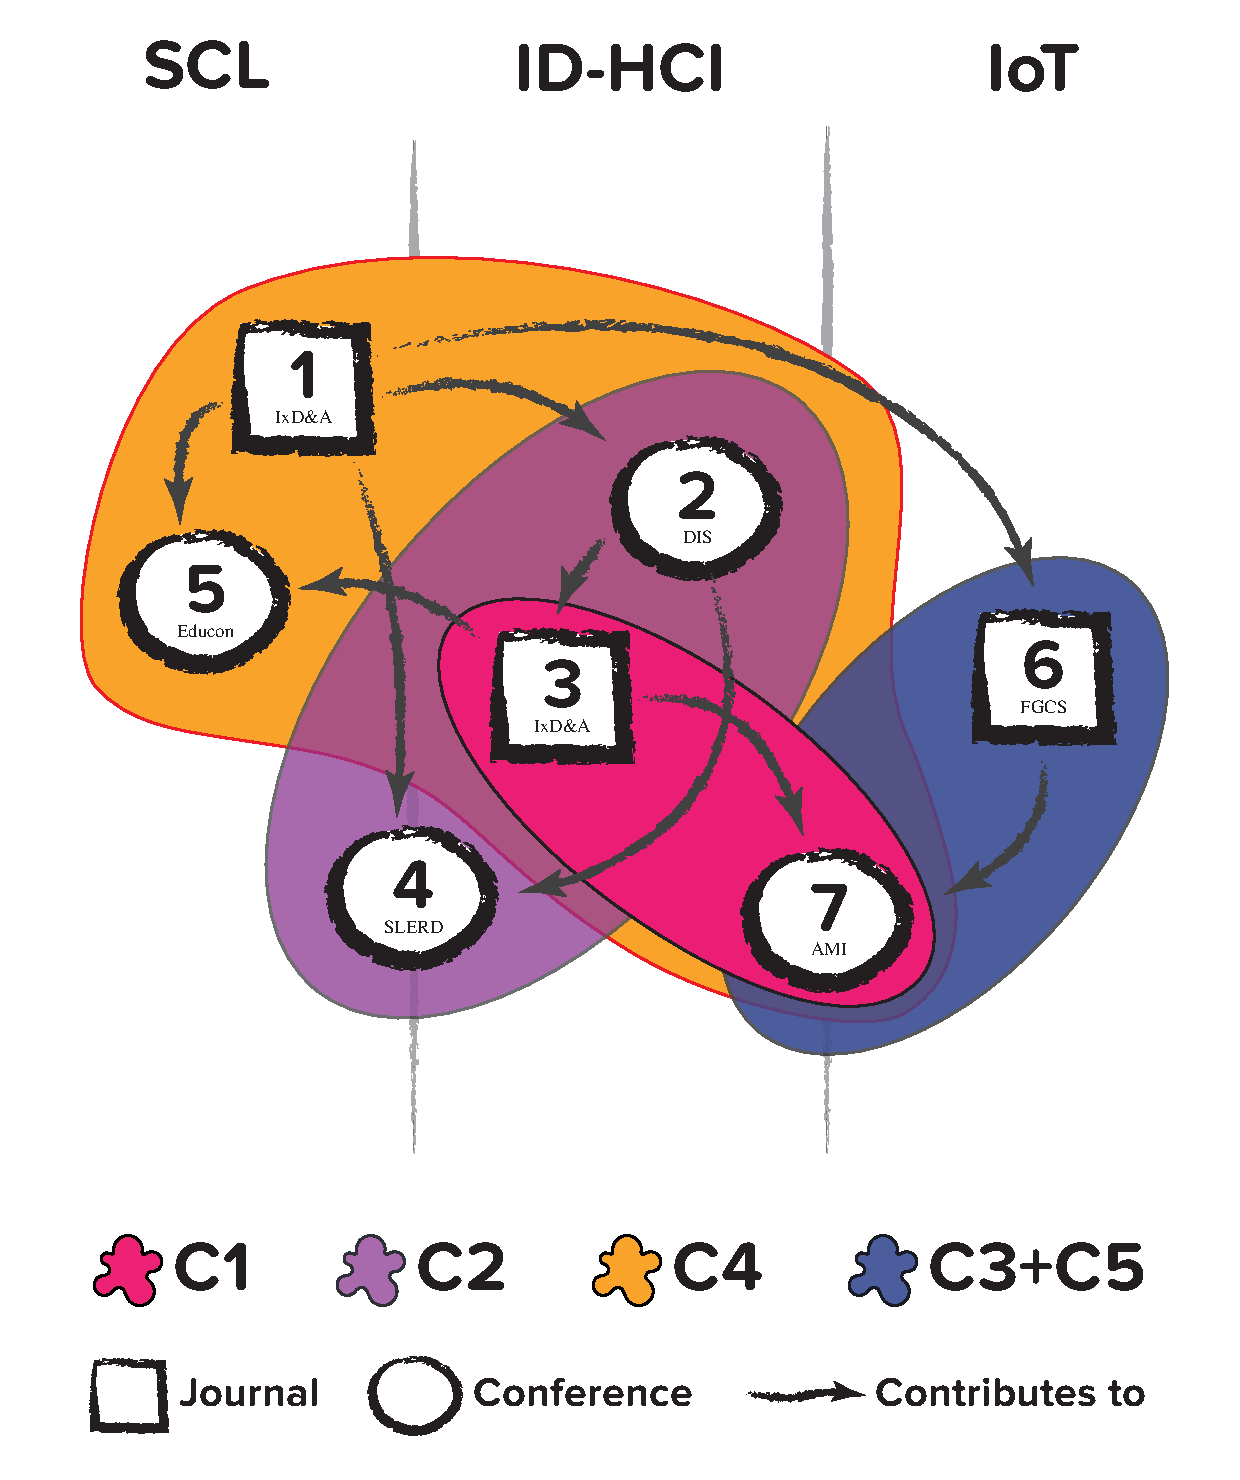
\includegraphics[width=\textwidth]{papers}
	\caption{A schema of the contributions. On top, from left to right: the domains of SCL, ID, HCI and IoT.}
	\label{fig:papers-contributions}
\end{figure}

\begin{table}[tbh]
	\centering 
	\caption{Mapping of contributions with papers.} 
	\label{tab:papers-and-contributions} 
	\smallskip
	\begin{tabular}{@{}lccccc@{}}
	\toprule
	  & C1 & C2 & C3 & C4 & C5 \\
	\midrule
	Paper 1 & & & & \textbullet & \\
	Paper 2 & & \textbullet & & \textbullet & \\
	Paper 3 & \textbullet & \textbullet & & \textbullet & \\
	Paper 4 & & \textbullet & & & \\
	Paper 5 & & & & \textbullet & \\
	Paper 6 & & & \textbullet & & \textbullet \\
	Paper 7 & \textbullet & & \textbullet & \textbullet & \textbullet \\
	\bottomrule 
	\end{tabular}
\end{table}


\section[C1: \Ci][Contribution 1]{C1: \Ci.}
\label{c1}

Contribution 1 is related to the theoretical definition, design and evaluation of an integrated framework supporting non-experts in idea generation and rapid prototyping of IoT applications based on augmented objects. In the context of this holistic process, the work presented in the thesis can be divided into two main blocks. The first one addresses the initial idea generation and design phases, where non-experts learn about the domain and generate an idea. The second block aims at creating a tangible prototype of the idea generated and includes the programming of the augmented object behaviour.
The process is tuned to be integrated, reusing the same conceptual building blocks during the different phases. It allows gradually building on the knowledge acquired, steadily supporting non-experts without demanding professional skills in any of the steps required. Special attention to the nature of this holistic process is reserved in P3 and P7, which also represent at best the work pertaining to each of the two blocks. For a detailed description of the complete framework, see Chapter~\ref{cha:iot-framework}.

This novel approach differs from the one adopted by most of the toolkits already available, which usually support either the design and brainstorming block or the prototyping and programming one, with no facilitation in bridging the two stages. A production-ready toolkit embracing this framework can be beneficial in education and design and for tangible exploration of creative ideas.


\section[C2: \Cii][Contribution 2]{C2: \Cii.}
\label{c2}

Contribution 2 of the thesis comprises new knowledge about how theoretical concepts of co-design and tangible user interaction (Chapter~\ref{cha:theory}) can inform the design, implementation and evaluation of a design and idea generation toolkit for IoT. The toolkit was developed during several design iterations. At the end of each iteration, the artefacts were empirically evaluated, and the feedback gathered informed the following version of prototypes. The final artefact produced by the work related to C2 was a new version of the Tiles ideation toolkit and its specialisation towards IoT applications for reflective learning and smart cities. The toolkit supports non-experts in idea generation and design of IoT applications; its initial version is described in P2. The design of the toolkit was refined during several iterations, in order to be frictionless and easy to adopt for users without previous knowledge of IoT or design methods. Some of the improvements and the specialisation towards the smart city domain are described in P3. Insights gathered on the field were also used to define a set of instructions and supporting material to guide the users during group-based brainstorming and design activities. I developed and refined such guidelines to provide a toolkit that is self-supported and does not need direct supervision by experts to be used. In order to facilitate adoption, especially in educational contexts, we designed the process to be self-contained, short-lasting from start to finish and entertaining. The toolkit, the idea generation process and all the materials were open source and were made available for free under a creative commons licence.

The Tiles ideation toolkit supports co-design as a strategy to involve different stakeholders in the brainstorming phase of an IoT solution. The group-based activity, the use of specific cards designed to spark creativity and reflection and the physicality of combining artefacts to define the seed of the idea all helped in provide a shared understanding of the problem and solution strategy, despite the diversities in skills and backgrounds of the participants. The toolkit is a viable instrument also for co-design workshops. Depending on the goal of the design workshop, a facilitator or expert might be necessary to support the users. This scenario emerged during the studies described in P4, where the toolkit was specialised towards IoT applications for reflective learning. Given the complexity of the approach for non-experts, a facilitator was needed to support the users during the workshops.

Contribution 2 can be a resource for researchers, designers, students and any user falling in the category of non-expert, who is interested in learning about IoT and generating ideas of IoT applications based on augmented objects and tangible interfaces. Although the toolkit was born to be generic, it was subsequently specialised for the smart city domain. This demonstrates its flexibility and the opportunity for it to be repurposed for other domains with limited effort.


\section[C3: \Ciii][Contribution 3]{C3: \Ciii.}
\label{c3}

The third contribution of the thesis includes the design, implementation and evaluation of an electronic and programming toolkit to prototype IoT ideas of augmented objects. The final prototypes produced are examples of tangible interfaces (Chapter~\ref{cha:theory}), and the toolkit itself is oriented into supporting rapid and tangible exploration of idea concepts. The RapIoT toolkit is designed to connect and build on the outcome of the brainstorming and design phases, covered by C2.
The RapIoT toolkit is composed of several hardware devices and software layers deployed in a cloud application, a development environment, a mobile app and a firmware for microcontrollers for embedded devices. For a more detailed description, see Chapter~\ref{cha:iot-framework}. The software structure of the toolkit is mainly described in P6, whereas a more extensive evaluation where non-experts created prototypes of augmented objects using the toolkit is reported in P7.
In order to allow non-experts to create a smart object and program its behaviour, the toolkit aimed to keep the entry barriers low, as in the preceding phases.
The toolkit includes electronic \textit{stickers} that can be attached to regular objects to provide sensing and actuation capabilities. Since several \textit{stickers} can be used in a single application, it is possible to prototype applications supporting distributed input and output, spread into several interconnected objects.
Ease of use and rapid deployment are guaranteed by the absence of any wire and the use of a simplified language for programming and by not requiring the installation of any software.

Contribution 3 can provide valuable insights into how to design a toolkit for tangible exploration of ideas for non-experts. The RapIoT toolkit itself is released under a creative commons licence and is free to use. It can act as a resource for non-experts, designers, students and makers. Crafting a physical prototype is an enriching experience that conveys knowledge, builds experience and provides a tangible artefact to validate use cases and idea concepts. Artefacts can also represent a shared means to further develop the discussion and collaboration around the original idea.


\section[C4: \Civ][Contribution 4]{C4: \Civ.}
\label{c4}

The fourth contribution of the thesis is related to the educational outcome, mainly connected to the use of the Tiles ideation toolkit during school hours, in the context of SCL. The user studies described in most of the papers included in this thesis had a twofold purpose: (i) to evaluate a specific iteration of the toolkit design and (ii) to support the learning process of the students involved in the evaluation. These user studies involved students aged from 13 to 27. The ideation workshop was included in the programme of courses on IoT or design or performed as a standalone activity during school hours.
While collecting data on the aspects related to the toolkit, we were also able to extend the investigation towards the learning outcome of the idea generation and prototyping activities supported by the toolkits. We recorded good feedback in terms of increased knowledge about the challenges connected to smart cities, the definition of IoT and its design space and increased interest in programming and tinkering.

Contribution 4 provides guidelines and an overview of the lessons learned while deploying the toolkits for educational purposes. Knowledge was gathered in adapting the creative activity to students at different levels and with diverse backgrounds.


\section[C5: \Cv][Contribution 5]{C5: \Cv.}
\label{c5}

The fifth contribution condenses the experience gathered in working with IoT design and prototyping toolkits and IoT systems in general. During the research activities described in this thesis, a considerable effort was made in experimenting with and investigating different IoT technologies, software frameworks, sensors, microcontrollers and networking solutions. Some of the outlined challenges affecting modern IoT solutions were identified, and the vision for an improved IoT technical framework was drafted, inspired and supported by emerging movements, standards and publications targeting the same shortcoming. Some of these challenges were broad and generic. However, whenever possible, the IoT model was specialised to address the requirements dictated by having non-experts as target users.

Contribution 5 provides the description of an IoT technical framework to support rapid prototyping of smart objects, having non-experts as target users. The envisioned solutions aim to be open, accessible and future-proof, following the philosophy adopted by the web. See Chapter~\ref{cha:iot-framework} for a more detailed description of the framework.